\chapter{Vývojová dokumentace}
Celá práce je rozdělena do dvou projektů Visual Studia. První z nich je \ccc{DungeonMasterParser}, 
který zajišťuje rozparsování herních dat \vref{level-parsing}. Celý tento projekt se skládá z~datových 
tříd odpovídající formátu souboru \ccc{DUNGEON.DAT} resp. \ccc{GRAPHICS.DAT} (viz sekce \ref{dungeon-objects} resp. \ref{dungeon-properties}),
které pak sestaví dohromady třída \ccc{DungeonParser} za vzniku objektu třídy \ccc{DungeonData}.
Při vytváření instance třídy \ccc{DungeonData} se pak provede načtení dat odpovídající soubor \ccc{DUNGEON.DAT}.
Kvůli tomu tento projekt referecuje knihovnu HTML Agility Pack \cite{HtmlAgilityPack}.

Druhý projekt \ccc{DungeonMasterEngine} obsahuje už samotný engine, kterému se bude hlavně věnovat tato kapitola.
Projekt s enginem pak referncuje projekt \ccc{DungeonMasterParser} a framework MonoGame \cite{MonoGame}.
Data týkající se herních úrovní jsou pak ve složce \ccc{/Data} a data jako textury, fonty nebo modely jsou ve složce
\ccc{/Content} jak je tomu MonoGame zvykem.  
Oba projekty se pak snaží dodržovat následující konvence:

\begin{itemize}
\item Každá třída nebo rozhraní jsou ve zvláštním souboru korespondujícím jejich názvu. (s výjimkou generických tříd se stejným názvem jako negenerické)
\item Skupiny třídy, které patří logicky k sobě se separují do zvláštních složek.
\item Jednotlivé složky odpovídají jemným prostorům.
\item Názvy rozhraní začínají písmenem \ccc{I}.
\item Třídy rozšiřující abstraktní třídy mají část jejich názvu.
\item K abstraktním třídám většinou existuje odpovídající rozhraní se stejnými položkami.
\end{itemize}

Následující sekce této kapitoly popisuje třídy reprezentující jednotlivé části enginu a vztahy mezi nimi.

\section{Jádro enginu -- \ccc{DungeonBase}}\label{engine-core-section}

Jádro enginu reprezentuje třída \ccc{DungeonBase} a skládá ze tří důležitých komponent, které do něj lze předat při jeho vytváření. 
Za těmito komponentami stojí následující rozhraní:

\begin{itemize}
\item \ccc{ILeader} -- reprezentuje hráče a jeho skupinu, kterou lze skrze něj ovládat.
\item \ccc{IFactories} -- obsahuje factories pro tvorbu předmětů, nepřátelských entit, kouzel, akcí a definuje úrovně osvětlení.
\item \ccc{IDungeonBuilder} -- vytváří pro engine herní úrovně.
\end{itemize}

Pro reimplementaci hry Dungeon Master jsou pak použity následující třídy \ccc{LegacyLeader},
\ccc{LegacyFactories}, \ccc{LegacyMapBuilder}. Konkrétní typy implementací rozhraní
\ccc{ILeader} a \ccc{IDungeonBase} lze předat jádru jako typové parametry.
Případný front end potom může skrze instanci jádra pracovat přímo s konkrétními typy \cc{frontend-core}. Tento projekt
neobsahuje žádné uživatelské rozhraní, namísto něho je pro udávání některých příkazu použita konzole \ccc{GameConsole}.

\imgx{frontend-core}{Ilustrace komunikace frondendu s jádrem enginu. }

\subsection{Asynchronní funkce}\label{async-engine}

Samotné jádro enginu je vytvořeno a aktualizováno ze třídy \ccc{Engine}, která je potomkem třídy \ccc{Game} zajišťující herní smyčku.
V řadě částí enginu se využívají asynchronní funkce ke zjednodušení implementace. Důležité je 
poznamenat, že tyto funkce předpokládají, že budou vykonávané v jednom vlákně - jinak může velmi jednoduše dojít k race condition.
Z toho důvodu je nutné přepnout chování asynchronních funkcí tak, aby se prováděli v jednom vlákně. To lze udělat nastavením 
vhodného synchronizačního kontextu v hlavním vláknu skrze funkci \ccc{SynchronizationContext.SetSynchronizationContext}. 
Tato funkce má jako parametr instanci třídy \ccc{SynchronizationContext}. Správnou implementaci synchronizačního kontextu 
-- tak aby se asynchronní funkce prováděli v jednom vlákně -- zajišťuje třída \ccc{GameSynchronizationContext}. Tento synchronizační
kontext je nastaven v konstruktoru třídy \ccc{Engine} a provádění asynchronních funkcí potom probíhá ve funkci \ccc{Engine.Update}.
K synchronizaci je použita fronta, kterou je nutné synchronizovat pomocí zámků.
V každém volání této funkce je vyprázdněna celá fronta asynchronních funkci, proto je třeba dávat pozor na její přehlcení,
které může v konečném důsledku vést až k neresponzivnosti aplikace.


\subsection{Správa herních úrovní a dlaždic}\label{engine-level-management}
Při inicializaci jádra je na objektu hráče zaregistrována událost \ccc{ILeader.LocationChanged}, která
je vyvolána po přesunu hráče na novou dlaždici. Zaregistrování resp. odregistrování události se provede po
přiřazení hodnoty do vlastnosti \ccc{Leader}. V obsluze této události se pak provede aktualizace
viditelných dlaždic pomocí funkce \ccc{UpdateVisibleTiles} \cc{core-tileUpdate}. K nalezení viditelných dlaždic tato funkce používá
třídu \ccc{RendererSearcher}, která je potomkem třídy \ccc{BreathFirstSearch}. Nalezené dlaždice se
uloží do protected proměnné \ccc{currentVisibleTiles}. V dalším kroku je zavolána funkce 
\ccc{SetupLevelConnectors}, jenž projde všechny viditelné dlaždice vedoucího do jiných úrovní. Pro
každou tuto dlaždici dojde pak voláním funkce \ccc{ConnectLevels} k propojení dané dlaždice s další
úrovní. Poslední akcí je přiřazení úrovně, v které se hráč vyskytuje, do proměnné \ccc{CurrentLevel}.

Funkce \ccc{ConnectLevels} načte danou úroveň pomocí funkce \ccc{LoadLevel}, která tak učiní skrze builder.
Načtená úroveň je pak uložena do kolekce \ccc{ActiveLevels}, ve které jsou vždy tři poslední úrovně.
Dlaždice, které propojují herní úrovně, by měli implementovat rozhraní \ccc{ILevelConnector}.
Funkce \ccc{ConnectLevels} pak nastaví cílovou dlaždici do vlastnosti \ccc{ILevelConnector.NextLevelEnter}.
Dlaždice implementující toto rozhraní by měla zajistit její propojení s dlaždicí \ccc{ILevelConnector.NextLevelEnter}.
Všechny funkce zmíněné v této sekci jsou virtuální, a proto je možné jejich chování upravit přetížením.

\imgx{core-tileUpdate}{Ilustrace funkce jádra. }

\subsection{Aktualizace a rendering}
MonoGame zajišťuje herní smyčku, skrze kterou je pak třeba na enginu volat funkce \ccc{Update} a \ccc{Draw}.

V každém zavolání funkce \ccc{Update} se provede aktualizace všech herních úrovní v kolekci \ccc{ActiveLevels}.
Herní úroveň reprezentuje typ \ccc{DungeonLevel}, který má v sobě uložené dlaždice, obtížnost a objekty vyžadující
aktualizaci -- které se u něj zaregistrovaly \vref{engine-core-section}. Funkce \ccc{DungeonLevel.Update} pak 
zavolá na všech zaregistrovaných objektech  funkci \ccc{IUpdate.Update}. Všechny tyto objekty musí implementovat
rozhraní \ccc{IUpdate} a musí se sami starat o odregistrování z kolekce, když už aktualizaci nevyžadují. Dále je volána 
funkce \ccc{ILeader.Update} na hráči. Při každém provedení aktualizace se ještě zavolá virtuální funkce 
\ccc{UpdateLight}. Proces reprezentuje obrázek \ref{core-update-draw}.

Funkce \ccc{UpdateLight} přiřadí do proměné \ccc{Light} hodnotu určující úroveň světla, která je v setteru
vlastnosti přepočítána na vzdálenost, po kterou se vykreslují dlaždice. Getter pak vrací již samotnou vzdálenost,
nikoliv hodnotu světla. Hodnota světla je 0 až 5, kde 0 reprezentuje největší osvětlení. Takto je to nastaveno
z důvodu kompatibility se zdrojovými kódy originální hry \cite{DMDecompilation}. 
 Funkce projde všechny šampiony v kolekci \ccc{ILeader.PartyGroup} a nalezne všechny 
objekty implementující rozhraní \ccc{ILightSource}. Na základě hodnot \ccc{ILightSource.LightPower} vypočte 
výslednou hodnotu osvětlení. Tento výpočet lze změnit přetížením funkce. 

V každém zavolání funkce \ccc{Draw} se potom provede vykreslení všech dlaždic v kolekci \ccc{currentVisibleTiles}
skrze jejich renderer \vref{renderer-interactor}. Dále jsou zavolány funkce \ccc{ILeader.Draw} pro vykreslení objektů
ve správě hráče a virtuální funkce \ccc{DrawMiniMap}, která provede vykreslení minimapy.

\imgx{core-update-draw}{Ilustrace aktualizace a vykreslování z pohledu jádra. }

\section{Dlaždice -- \ccc{ITile}}
Nejobecnější strukturu dlaždice definuje rozhraní \ccc{ITile}. Každá dlaždice musí mít definované sousedy,
to zajišťuje položka \ccc{Neighbors} typu \ccc{TileNeighbors}. Tento typ implementuje rozhraní \ccc{INeightbors},
které vyžaduje pouze enumerátor dvojic se směrem a dlaždicí. Směr reprezentuje struktura \ccc{MapDirection}, kde
se jednotlivé směry dají získat skrze její statické členy. Třída \ccc{TileNeighbor} potom implementuje ještě
pomocné funkce a vlastnosti pro jednoduší práci se sousedy. Pomocí této vlastnosti se objekty mohou pohybovat
mezi dlaždicemi \cc{layout-reserve}. Po vstupu objektu na dlaždici je třeba zavolat na předchozí dlaždici funkci \ccc{OnObjectLeft} a
na nové dlaždici funkci \ccc{OnObjectEntered}. Díky tomu může dlaždice reagovat na vstup resp. odchod objektů --
což je použité například pro přepínače na podlaze. Další vlastností dlaždice je \ccc{LayoutManager}, který 
musí používat entity při pohybu po dlaždicích a mezi nimi. \ccc{LayoutManager} je třída poskytující správu prostoru
na dlaždici, tak aby každý prostor zaujímala pouze jedna entita \vref{layout-manager-section}. Před pohybem entity je
tedy ještě třeba zarezervovat skrze \ccc{LayoutManager} cílový prostor na dlaždici a po dokončení pohybu
je naopak třeba uvolnit prostor předchozí. Poslední položkou potřebnou pro pohyb mezi dlaždicemi je vlastnost
\ccc{IsAccessible}, která určuje, zda lze na dlaždici vstoupit.

\imgx{layout-reserve}{Ilustrace pohybu mezi prostory a dlaždicemi. }

Pro implementaci funkce přepínačů je třeba zajistit komunikaci mezi dlaždicemi \vref{actuator-message-representation}.
Za tímto účelem obsahuje dlaždice vlastnosti pro změnu jejího stavu. Buď lze obsah dlaždice aktivovat přímo
pomocí funkce \ccc{ActivateTileContent} resp. \ccc{DeactivateTileContent} nebo pomocí zaslání zpráv, k jejichž
příjetí slouží funkce \ccc{AcceptMessageBase}. Konkrétní stav je obsahuje pak vlastnost \ccc{ContentActivated}.


V poslední řadě rozhraní reprezentující dlaždice obsahuje prvky: 
\begin{itemize}
\item \ccc{Position} -- absolutní pozice od počátku souřadnic,
\item \ccc{GridPosition} -- souřadnice dlaždice na mřížce, 
\item \ccc{Drawables} -- do této kolekce se mohou zaregistrovat objekty implementující rozhraní \ccc{IRenderable}, 
	které se nechtějí registrovat u dlaždice pomocí funkcí pro vstup a výstup a zároveň se potřebují renderovat, 
\item \ccc{ObjectEntered} resp. \ccc{ObjectLeft} -- události vyvolané při vstupu resp. odchodu objektu,
\item \ccc{Level} -- reference na level, ve kterém se dlaždice nachází,
\item \ccc{IsInitialized} -- určuje, zda je dlaždice plně inicializovaná \vref{level-inicialization},
\item \ccc{Initialized} -- tato událost je dlaždicí vyvolána pouze jednou a to v momentě, kdy jsou všechny její části inicializované.
		Tuto událost využívají živé entity k určení doby jejich obživnutí.
\end{itemize}


\subsection{Inicializace dlaždic}
Jak již bylo zmíněno v analýze \vref{level-inicialization}, k inicializaci dlaždic jsou použity tzv. inicializátory. Inicializátor
obsahuje vlastností, které by normálně byly předány jako parametry v konstruktoru. Ovšem v moment předávaní
inicializátoru do konstruktoru, inicializátor ještě nemusí mít naplněné všechny hodnoty. Namísto toho má události \ccc{Initializing}
resp. \ccc{Initialized}, které jsou vyvolány při resp. po inicializaci. Na tuto událost je třeba zaregistrovat
inicializační funkci, která zkopíruje data z inicializátoru do samotného objektu. Pro každou úroveň hierarchie
dědičnosti jsou určeny zvláštní vlastnosti a zvláštní inicializační události. Rodičovské události  inicializátoru jsou vždy
po zdědění rodičovského inicializátoru zakryty novými inicializačními událostmi pro danou úroveň dědičnosti.
Tento způsob je použit pouze pro inicializaci dlaždic. Pro jiné objekty, může inicializátor sloužit pouze jako 
objekt udržující parametry, které jsou hned v konstruktoru inicializované. 

\subsection{Implementace dlaždic}
Částečnou implementaci rozhraní \ccc{ITile} zajišťuje abstraktní třída \ccc{Tile}, která definuje virtuálně \ccc{LayoutManager}.
Dále abstraktně deklaruje kolekci \ccc{SubItems}, která obsahuje všechny objekty na dlaždici. Objekty, které 
implementují rozhraní \ccc{IRenderable}, jsou potom skrze tuto kolekci vykreslovány.
Dlaždice také má tzv. strany, a jsou to buď stěny, strop nebo podlaha \cc{tile-sides}.
Pro tyto strany pak abstraktně deklaruje kolekci \ccc{Sides}, jejímž stěnám pak přeposílá
případné zprávy, které přišly na tuto dlaždici skrze metodu \ccc{AcceptMessageBase}.
Dále implementuje také funkce \ccc{OnObjectEntered} resp. \ccc{OnObjectLeft} tak, že vyvolá jejich odpovídající událost.
Proto je pří případném přetížení těchto funkcí v potomkovi nutné zavolat implementaci rodiče. Všechny
předchozí popsané funkce je možné přetěžovat v potomkovi, a tak přizpůsobit prováděné akce.
V poslední řadě se tento inicializátor stará o inicializaci pozic na mřížce, úrovně a sousedů skrze \ccc{TileInicializator}. 

\imgx{tile-sides}{3D ilustrace dlaždice a jejích stran.}

Přímý generický potomek předchozí třídy \ccc{Tile\textlangle TMessage\textrangle}, kde \ccc{TMessage} je alespoň \ccc{Message},
poskytuje možnost přijímat v potomcích zprávy vlastního typu \vref{actuator-representation}. V případných potomcích teto třídy 
lze naimplementovat funkci \ccc{AcceptMessage}, která přijímá zprávy typu \ccc{TMessage}. Tato třída přetěžuje a zároveň 
uzavírá metodu \ccc{AcceptMessageBase} tak, že deleguje zprávy typu \ccc{TMessage} do metody \ccc{AcceptMessage}. 
Naopak základní implementace metody \ccc{AcceptMessage} je zavolání právě rodičovské implementace \ccc{AcceptMessageBase}. 
Při případném přetěžování této funkce je třeba rozhodnout, zda je nutné volat implementaci rodiče. Všechny dlaždice,
které dědí ze třídy \ccc{Tile\textlangle TMessage\textrangle}, vytváří dva potomky. První z nich je pro případné rozšiřitele,
a proto ponechává typový parametr, druhý pak specifikuje typový parametr na obecný typ \ccc{Message}.

\subsubsection{Dlaždice podlaha -- \ccc{FloorTile\textlangle TMessage\textrangle}}
Tato dlaždice implementuje funkci všech jejích stran \cc{tile-sides}. Na stranách, kde
nemá dlaždice sousedy jsou přidány stěny, které mají podporu pro přepínače \vref{dungeon-objects} a dekorace \vref{actuator-analyza}.
Dále je přidána strana na místo stropu a podlahy. Na stranu s podlahou pak může obsahovat přepínač a je na ni možné odkládat
či z ni odebírat předměty. Dlaždice také deleguje veškeré vstupy resp. odchody objektů do samotné strany podlahy
typu \ccc{FloorSide} \vref{tile-sides-section} a to kvůli podpoře odkládání předmětů na zem.

\subsubsection{Další implementace dlaždic}
Další dlaždice převážně využívají dědičností dlaždici podlahy. Výjimkou jsou například schody,
které jsou zároveň příkladem dlaždice implementující rozhraní \ccc{ILevelConnector}. Engine při načtení 
levelu nastaví vlastnost \ccc{ILevelConnector.NextLevelEnter} na odpovídající dlaždici \vref{engine-level-management}.
Při změně předchozí vlastnosti provede dlaždice nastavení sousedů vedoucích do dalšího levelu a používá k tomu vlastní 
implementaci sousedů přetížením vlastnosti \ccc{Neighbors}. Tato možnost je použita ještě u jámy, kvůli propadu do nižšího levelu. 
Rozhraní spojující levely je ještě použito u teleportu, kde při vstupu správného objektu na teleportační dlaždici 
dojde k teleportaci objektu na dlaždici \ccc{ILevelConnector.NextLevelEnter}. Další dlaždicí jsou dveře, které opět 
dědí z podlahy a navíc implementují rozhraní \ccc{IHasEntity}. Toto rozhraní obsahuje vlastnost typu \ccc{Entity},
která reprezentuje neživou entitu na dlaždici. S touto entitou můžou pak pracovat akce, kterými lze dveře rozbít.
Poslední dlaždici reprezentuje třída \ccc{LogicTile}, na kterou nelze vstoupit a slouží pouze jako podpora
pro přepínače \vref{actuators-implementation}.

\subsection{Strany dlaždic -- \ccc{ITileSide}}\label{tile-sides-section}
Jak již bylo naznačeno \cc{tile-sides}, dlaždice mohou mít strany, které jsou buď stěny, podlaha nebo strop.
Každou tuto stranu reprezentuje samostatný objekt, který má svůj renderer-interactor \vref{renderer-interactor}. 
Toto rozhraní vyžaduje pouze položku pro renderer a funkci pro přijímání základních zpráv \ccc{Message}. 
Tato funkce je zde z kompatibilních důvodu s originální hrou, kdy texty na zdech mohou být těmito 
zprávami skryty či zobrazeny.

Následuje seznam jednotlivých implementací:
\begin{itemize}

\item \ccc{TileSide} -- reprezentuje pouze holou stěnu bez žádných funkcí, která obsahuje
	pouze vlastnost typu \ccc{MapDirection} určující její pozici. 

\item \ccc{ActuatorTileRenderer} -- přímý potomkem předchozí strany, který navíc obsahuje přepínač a renderer, 
	jenž se navíc stará o jeho vykreslování a interakci. 

\item \ccc{TextTileSide} -- opět přímý potomek první strany, jejíž renderer navíc zobrazuje na zdi text. Viditelnost textu lze změnit zasláním zprávy
	této straně. 

\item \ccc{FloorTileSide} -- tato strana obsahuje čtyři úložiště,
na které může hráč pokládat předměty. Je to jedno z míst, kde je potřeba komunikovat s rodičovskou dlaždicí, k tomu
slouží událost \ccc{SubItemsChanged}, která se vyvolá vždy, když byl nějaký předmět odebrán nebo přidán.
Pomocí enumerátoru tohoto objektu je potom možné získat obsažené objekty. Předměty lze pak na podlahu přidávat dvěma 
způsoby, přičemž oba pomocí události informují rodičovskou dlaždici o změně jejího obsahu. První možností je položení 
předmětu přímo z ruky hráče pomocí renderer-interactoru. Druhý způsob je zavolání metody \ccc{OnObjectEntered} resp. \ccc{OnObjectLeft} 
objevující se například při teleportaci nebo hodu předmětu. Celou situaci zobrazuje obrázek \ref{floor-side}.

\item \ccc{ActuatorFloorTileSide} -- přímý potomek předchozí strany podlahy, který navíc přidává na podlahu nášlapný přepínač.

\end{itemize}

\imgx{floor-side}{Ilustrace komunikace podlahy s její dlaždicí při přidávání předmětu.}

\section{Přepínače -- \ccc{IActuatorX}}\label{actuators-implementation}

Za přepínači stojí rozhraní \ccc{IActuatorX}, které vyžaduje pouze API pro příjem zpráv typu \ccc{Message} -- pro dodržení
kompatibility s původní hrou. Toto rozhraní pak implementuje třída \ccc{ActuatorX}, která reprezentuje přepínače používající 
pro jejich funkci senzory z originální hry \vref{actuator-analyza}. Kromě toho dále existují implementace přepínačů, které jsou provedeny
jiným způsobem.

\subsection{Implementace obecných přepínačů}
Tato sekce pojednává o přepínačích, které ke své funkci nepoužívají senzory. V tomto enginu jsou použity pro 
dekorace, které provádějí nějakou funkci. K těmto dekoracím v originální hře nenáleží žádné senzory. 
Studií dekompilovaného kódu originální hry \cite{DMDecompilation} se ukázalo, že některé akce jsou fixovány 
na konkrétní typy dekorací. Například pro dekorace s výklenky je naimplementována možnost vkládaní předmětů.
Jelikož tyto dekorace mohou být i součástí senzorů, bylo zapotřebí, aby objekty reprezentující dekorace
implementovali rozhraní \ccc{IActuatorX}, a tak bylo možné naimplementovat funkce pro jejich interakci.

U těchto přepínačů lze zvolit jejich vnitřní formát. Existující implementace jsou:
\begin{itemize}
\item \ccc{DecorationItem} -- stará se pouze o rendering dekorace, který zajišťuje třída \ccc{DecorationRenderer}. 
\item \ccc{Alcove} -- reprezentuje dekoraci výklenku, o jehož rendering a interakci se stará třída \ccc{AlcoveRenderer}. 
\item \ccc{ViAltairAlcove} -- potomek třídy \ccc{Alcove}, který se navíc stará o reinkarnaci šampionů.
\end{itemize}

\subsection{Implementace přepínačů se senzory}
Tyto přepínače se skládají z řady senzorů, které mohou provádět následující akce:

\begin{itemize}
\item změna stavu vzdálené dlaždice,
\item zarotování sekvencí senzorů přepínače \cc{actuator-rotation},
\item přidání zkušeností hráči.
\end{itemize}

Při pokusu o aktivaci přepínače dojde postupně, k aktivaci všech jeho senzorů.
Senzory pak mohou být aktivovány následujícími způsoby:

\begin{itemize}
\item kliknutím myši na dekoraci senzoru, pokud je senzor na zdi, 
\item vstupem resp. odchodem hráčovi skupiny na dlaždici resp. z dlaždice, 
\item zprávou vyslanou jiným senzorem.
\end{itemize}

Více viz sekce \ref{actuator-analyza}.

\subsubsection{Implementace senzorů}

Každý typ senzoru má jinou podmínku aktivace. Senzory se dělí na senzory použité na podlaze, zdi a
na speciální tzv. logické senzory.

Hlavní třídou reprezentující senzor je abstraktní třída \ccc{SensorX}. Tato třída obsahuje společné funkce,
které jsou využívány jejími potomky. Dále také definuje vlastnosti, které lze rozdělit do tří skupin.
Tyto vlastnosti jsou inicializovány inicializátorem \vref{level-inicialization}, který slouží pouze jako datový nosič.
Jde o inicializátor, který reprezentuje třída \ccc{SensorInitializerX}. Pro inicializaci potomků jsou 
používány poděděné implementace tohoto inicializátoru.

Vlastnosti senzorů třídy \ccc{SensorX}:
\begin{itemize}
\item Obecné vlastnosti:
	\begin{itemize}
	\item \ccc{Delay} -- opoždění akce v milisekundách, po kterém se provede akce senzoru.
	\item \ccc{LocalEffect} -- informace, zda-li je akce určena lokálně pro rodičovskou dlaždici nebo pro vzdálenou.
	\item \ccc{OnceOnly} -- informace, zda-li je senzor možné aktivovat pouze jednou.
	\item \ccc{RevertEffect} -- u většiny přepínačů obrátí efekt výsledné akce, nicméně přesný význam si stanový vždy konkrétní senzor. 
	\item \ccc{Audiable} -- informace určující, zda po aktivaci dojde k přehrání zvuku.  (v tomto enginu není použit)
	\item \ccc{GraphicsBase} -- reprezentuje dekoraci a zároveň přepínač obecného typu implementující rozhraní \ccc{IActuatorX}.
			Pokus o aktivaci tohoto přepínače se provádí pouze pokud je zobrazena dekorace \cc{decoration-actuator}.
	\end{itemize}

\item Vlastnosti pro lokální akci:
	\begin{itemize}
	\item \ccc{Rotate} -- informace určující, zda-li se má seznam senzorů při aktivaci zarotovat \cc{actuator-rotation}.
	\item \ccc{ExperienceGain} -- informace určující, zda-li se mají hráči po aktivaci přidat zkušenosti.
	\end{itemize}

\item Vlastnosti pro vzdálenou akci:
	\begin{itemize}
	\item \ccc{Effect} -- určuje jaká zpráva je odeslaná na cílovou dlaždici.  (Akce zprávy může být obrácená pokud je nastavena vlastnost \ccc{RevertEffect}).
	Hodnoty efektu jsou následující:
		\begin{itemize}
		\item Aktivace 
		\item Deaktivace
		\item Přepnutí stavu
		\item Drž -- tento stav nelze odeslat ve zprávě a je na senzoru, aby ho interpretoval pomocí aktivace či deaktivace.
		\end{itemize}
	\item \ccc{Specifier} -- směr použitý v odeslané zprávě, který může být interpretován jako číslo (lze získat pomocí \ccc{MapDirection.Index}).
	\item \ccc{TargetTile} -- reference na cílovou dlaždici.
	\end{itemize}
\end{itemize}

Kromě předchozích vlastností obsahuje tato třída funkce pro vykonání akcí senzorů. Pokud je efekt senzoru vzdálený, funkce  \ccc{TriggerEffect} odešle zprávu 
na danou cílovou dlaždici. Jinak provede akci pro lokální efekt, který lze 
také vykonat přímo zavoláním funkce \ccc{TriggerLocalEffect}. Tyto funkce lze použít pouze v potomcích.

Následující třídy jsou přímými potomky třídy \ccc{SensorX}:

\begin{enumerate}
\item\label{floor-tile-sensor} \ccc{FloorSensor} - tyto senzory lze vložit pouze do přepínačů, které mohou být na podlaze.
\item\label{wall-tile-sensor} \ccc{WallSensor} - tyto senzory lze vložit pouze do přepínačů, které mohou být na stěně.
\item \ccc{LogicGateSensor} resp. \ccc{CounterSensor} - pro tyto senzory existuje speciální dlaždice \ccc{LogicGateTile}
\end{enumerate}

Senzory z bodu \ref{floor-tile-sensor} a \ref{wall-tile-sensor} mají funkci \ccc{TryTrigger}, která se pokusí senzor 
aktivovat a pokud uspěje, stará se o provedení efektu. Zda-li se senzor aktivuje stanoví abstraktní funkce \ccc{TryInteract},
kterou implementují potomci. Pro každou variantu senzoru mají funkce odlišné parametry. Pokud je třeba modifikovat způsob 
provedení výsledného efektu, je možné funkce \ccc{TryTrigger} přetížit.

Kromě předchozích senzorů ještě existují tzv. logické senzory (viz \ref{floor-tile-sensor}). První z nich \ccc{LogicGateSensor} funguje 
jako logické hradlo, které má k dispozici osm bitů. Čtyři z nich jsou nastaveny při designu na hodnoty a ostatní na nuly. 
S druhou čtveřicí lze pak manipulovat pomocí zpráv. Index směru zprávy určuje kolikátý bit se má ovlivnit. A tento bit
je pak ovlivněn akcí zprávy. Pokud jsou obě čtveřice stejné, je vyvolán efekt senzoru. Dalším
senzorem je \ccc{CounterSensor}, který má dané číslo. Aktivační zprávy toto číslo poté navyšují a deaktivační zprávy
ho snižují. Pokud je číslo  nula, je vyvolán efekt.
 
\subsubsection{Implementace přepínačů používající senzory}

Rodiči těchto přepínačů je třída \ccc{Actuator}. Tato třída poskytuje funkci pro zarotování senzory přepínače, která
lze vyvolat pouze z potomků. Zda-li se mají senzory zarotovat se určuje nastavením vlastnosti \ccc{Rotate}, která se po jeho 
provedení nastaví zpět na false. Samotné zarotování se pak provede zavoláním funkce \ccc{ProcessRotationEffect}.

Prvním potomkem předchozí třídy je třída \ccc{FloorActuator}, která může obsahovat pouze senzory určené
na podlahu tj. \ccc{FloorSensor}. Pokus o její aktivaci se provádí funkcí \ccc{Trigger}. Jako první parametr se jí předává objekt,
který vstupuje resp. odchází z dlaždice, dále seznam všech objektů na dlaždici a naposled informace, zda objekt
vstupuje či odchází. Pro přepínač je vytvořena speciální podlaha \ccc{ActuatorFloorSide}, která se stará 
o volání funkce \ccc{Trigger}.

Dalším potomkem je třída \ccc{WallActuator}, která může obdobně obsahovat pouze senzory určené na zeď tj. \ccc{WallSensor}.
Pokus o její aktivaci se provádí opět funkcí \ccc{Trigger}, která má jediný parametr typu \ccc{ILeader}. Pro přepínač
je určena strana \ccc{ActuatorWallTileSide}. Funkce \ccc{Trigger} je pak volána skrze renderer dané strany. 
Tato se pak pokusí postupně aktivovat všechny senzory a navíc se pokusí aktivovat přepínač zobrazené dekorace \cc{decoration-actuator}.

\imgx{decoration-actuator}{Ilustrace struktury přepínače se senzory.}

Poslední speciální implementací je třída \ccc{LogicActuator}, která může obsahovat logické senzory.
Komunikace se senzory probíhá pomocí zasílání zpráv. Pro tento přepínač je vytvořena speciální dlaždice,
na kterou nelze hráčem vstoupit. Tato dlaždice je reprezentována třídou \ccc{LogicTile}. 

\begin{figure}[H]\centering
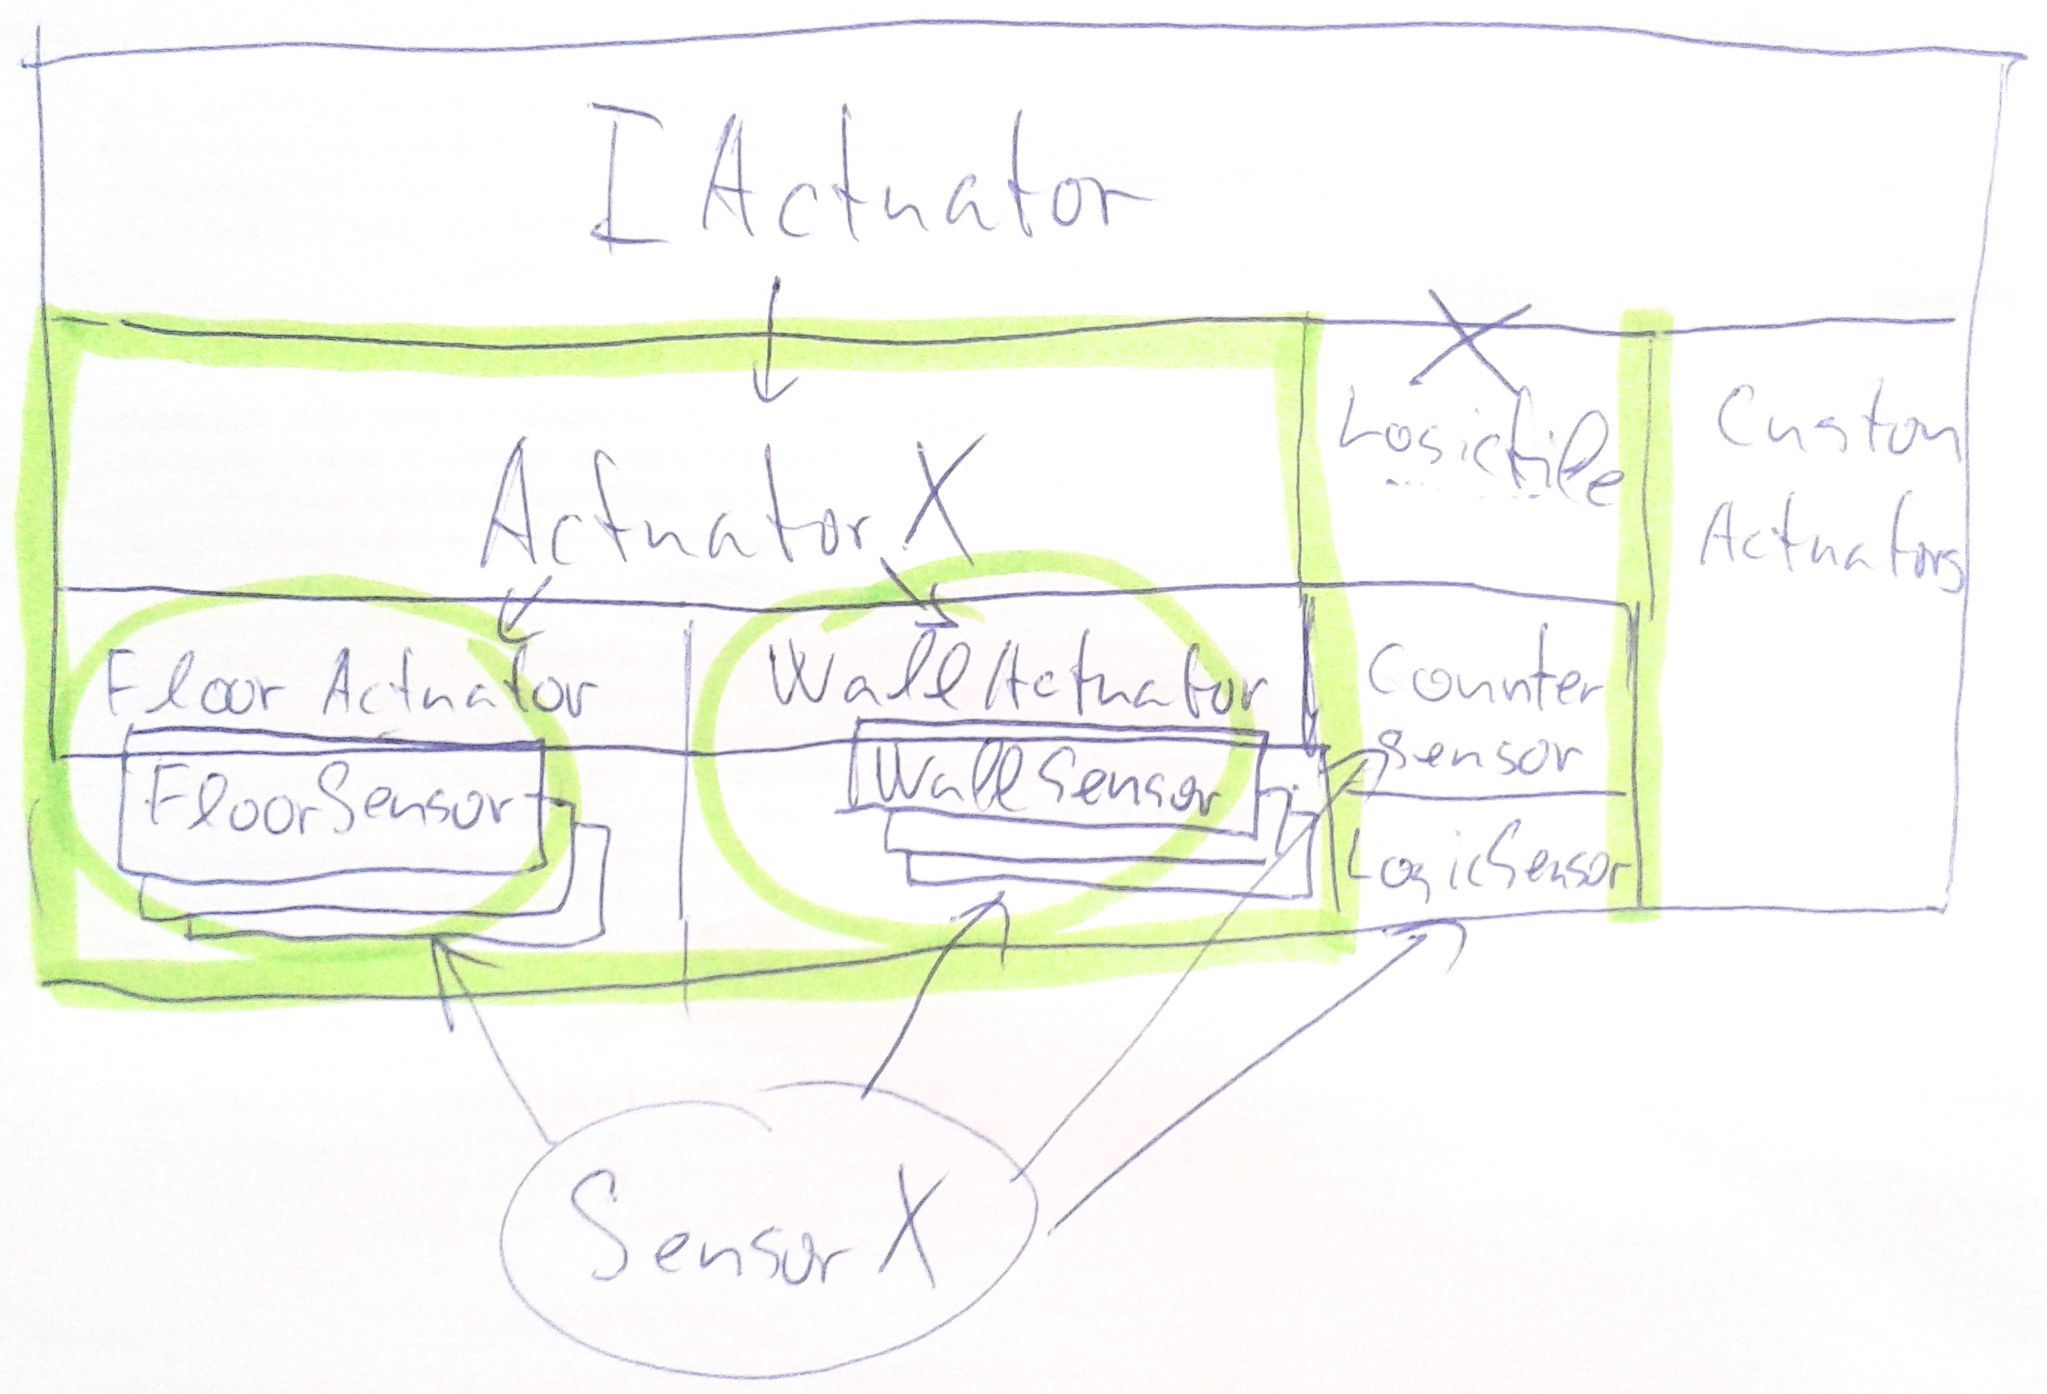
\includegraphics[width=\textwidth]{./img/actuator-sensor-hierarchii.png}
\caption{Ilustrace hierarchie přepínačů a senzorů.}
\label{actuator-sensor-hierarchii}
\end{figure}

\section{Herní entity}

Za deklarací neživých entit stojí rozhraní \ccc{IEntity}, které definuje funkci \ccc{GetProperty} pro získání vlastnosti dané entity.
Za živými entitami stojí naopak rozhraní \ccc{ILiveEntity}, která navíc disponuje funkcí \ccc{GetSkill} pro získání schopností. Dále
také deklaruje:

\begin{itemize}
\item tělo entity
\item způsob rozmístění entity na dlaždici
\item relace s dalšími entitami
\end{itemize}

\subsection{Implementace vlastností entit}

Vlastnost deklaruje rozhraní \ccc{IProperty}, které obsahuje následující atributy:
\begin{itemize}
\item \ccc{Value} -- stanovuje aktuální hodnotu dané vlastnosti, v jejím getteru a setteru se typicky provádějí 
	kontroly okrajových hodnot a případné reakce na ně.
\item \ccc{BaseValue} -- maximální hodnota, které může vlastnost nabýt, pokud není nějak modifikovaná.
\item \ccc{MaxValue} -- určuje maximální hodnotu včetně modifikací. 
\item \ccc{AdditionalValues} -- je to kolekce typů \ccc{IEntityPropertyEffect} obsahující modifikace dané vlastnosti.
\item \ccc{Type} -- je to vlastnost typu \ccc{IPropertyFactory}, která reprezentuje typ vlastnosti. Entita na základě 
	tohoto typu potom vrací odpovídající vlastnost. Pro usnadnění tvorby unikátních typů existuje generická třída \ccc{PropertyFactory}, 
	která má jako typový parametr typ alespoň \ccc{IProperty}. Tato třída se řídí vzorem singleton, jejíž jediná instance 
	lze získat přes statickou položkou \ccc{Instance}. Takto lze pak generovat typy pomocí třídy reprezentující vlastnost.
\end{itemize}

Pro usnadnění práce existuje implementace rozhraní \ccc{IProperty} a to třída \ccc{Property}. Tato třída definuje 
maximální hodnotu jako součet základních hodnoty a sumu modifikujících hodnot. Dále při nastavení konkrétní hodnoty ořezává
hodnotu do povoleného intervalu, který je mezi nulou a maximální hodnotou. Také definuje událost vyvolanou při změně hodnoty.
Všechny vlastnosti jsou deklarovány abstraktně nebo virtuálně. 

Některé vlastnosti mohou požadovat přístup k jiným vlastnostem či přístup k rodičovské entitě. V takovém
případě je na programátorovi, jak takového cíle dosáhne. Typicky se v takovém případě předá v konstruktoru
potřebná vlastnost nebo se vytvoří událost, která danou závislost deleguje vně. 

Seznam předdefinovaných vlastností je možné najít ve jemném prostoru \ccc{DungeonMasterEngine.DungeonContent.Entity.Properties}.
Jak již bylo zmíněno \vref{entity-properties}, může nastat, že daná entita vlastností nedisponuje. V takovém případě 
je vrácena instance třídy \ccc{EmptyProperty}. 

\subsection{Implementace dovedností entit}

Dovednosti deklaruje rozhraní \ccc{ISkill}, které obsahuje následující atributy:
\begin{itemize}
\item \ccc{SkillLevel} -- udává úroveň, na které je daná dovednost včetně úrovní získaných kouzelnými předměty.
\item \ccc{BaseSkillLevel} -- udává úroveň bez úrovní získaných kouzelnými předměty.
\item \ccc{Experience}  -- určuje celkovou dosavadní hodnotu zkušeností.
\item \ccc{TemporaryExperience} -- určuje dočasné zkušenosti, které můžou být jak přidávány tak odebírány.
\item \ccc{BaseSkill} -- je reference na základní dovednost \vref{analysis}. Pokud je daná schopnost 
	již základní, je hodnota \ccc{null}.
\item \ccc{AddExperience} --  umožňuje přidat zkušenosti.
\item \ccc{Type} -- je to vlastnost typu \ccc{ISkillFactory}, která reprezentuje typ dovednosti.  Entita na základě 
	tohoto typu potom vrací odpovídající dovednost. Stejně jako u vlastností, je možné tyto reprezentanty vytvářet pomocí generické třídy \ccc{SkillFactory}. 
\end{itemize}

Konkrétní algoritmus přepočítávání zkušeností na úrovní dovedností záleží vždy na konkrétní implementaci.  

Třída \ccc{SkillBase} implementuje získávání zkušeností schopností jako v originální hře. Všechny schopnosti 
využívající tuto třídu jsou ve jemném prostoru \ccc{DungeonMasterEngine.DungeonContent.Entity.Skill}. Stejně jako
u vlastností i zde entita nemusí mít dotazovanou schopnost. V takovém případě vrací instanci třídy \ccc{EmptySkill}.

\subsection{Tělo -- \ccc{IBody}}

Následující API umožňuje pro entity vytvořit různé druhy těl.
Tělo se skládá z částí, které mohou sloužit jako úložiště. Dále pak existují externí
úložiště tzv. inventáře. API je navržené tak, aby dovolovalo definovat různé druhy úložišť a těl. 
Engine obsahuje pouze implementaci pro lidské tělo tj. třída \ccc{HumanBody}.
Tělo entity je definováno rozhraním \ccc{IBody} a obsahuje následující atributy:

\begin{itemize}
\item \ccc{BodyParts} -- obsahuje seznam částí těla,
\item \ccc{Storages} -- obsahuje seznam všech úložišť včetně částí těla,
\item \ccc{GetStorage} -- funkce pro vyhledání úložiště včetně částí těla,
\item \ccc{GetBodyPart} -- funkce pro vyhledání části těla. 
\end{itemize}

\subsubsection{Externí úložiště -- \ccc{IInventory}}
Každý inventář má definovanou vlastnost \ccc{Type}, což je typ úložiště, který reprezentuje instance třídy 
implementující rozhraní \ccc{IStorageType}. Dále pak definuje readonly kolekci \ccc{Storage} pro ukládání předmětů.
A v poslední řadě obsahuje funkce pro přidávaní a odebírání předmětů z úložného prostoru tj. \ccc{TakeItemFrom}, \ccc{AddItemTo}, \ccc{AddItem},
\ccc{AddRange}. Třída \ccc{Inventory} implementuje všechny funkce inventáře a je jí tedy možno přímo použít nebo rozšířit.

\subsubsection{Část těla -- \ccc{IBodyPart}}
Část těla je definovaná rozhraním \ccc{IBodyPart}, které je potomkem rozhraní \ccc{IInventory}. Toto rozhraní navíc definuje 
následující vlastnosti: 
\begin{itemize}
\item \ccc{IsWound} -- definuje, zda je část těla zraněna,
\item \ccc{InjuryMultipler} -- definuje pravděpodobnost zranění části těla.
\end{itemize}

Obecnou implementací rozhraní je třída \ccc{BodyPart}. 

\subsection{Rozmístění entity na dlaždici}\label{layout-manager-section}

Rozhraní \ccc{IGroupLayout} definuje obecně možné rozmístění na dlaždici. Jeho vlastnost \ccc{AllSpaces} obsahuje všechny možné prostory, které daná entita může využít.
Toto prostory rozdělují prostor dlaždice na mřížku \cc{space-grid}, která nemusí být rovnoměrná.
Jednotlivě prostory jsou reprezentovány rozhraním \ccc{ISpace}. Dale API vyžaduje funkci \ccc{GetToNeighbour}, která nalezne cestu skrze prostory
na cílovou sousední dlaždici \cc{space-route}. Funkce \ccc{GetToSide} vrací cestu k libovolné ze stran dlaždice. Jednotlivé články cesty jsou 
reprezentovány rozhraním \ccc{ISpaceRouteElement}. Poslední funkce musí umět vytvořit z prostoru a dlaždice článek cesty,
tedy \ccc{ISpaceRouteElement}.  

\imgx{space-grid}{Ilustrace rozdělení dlaždice na prostory. }

Rozhraní \ccc{ISpace} musí definovat, jakým stranám dlaždice je prostor přilehlý. Dále musí pomocí obdélníku definovat prostor, který na dlaždici využívá.
Celý prostor dlaždice je pak definovaný na pole o velikosti 1000x1000. Přičemž souřadnice rostou
shora dolů a zleva doprava. Nahoře je pak sever, vpravo východ, dole jih a vlevo západ. Kromě toho také musí definovat sousední
prostory, k čemuž využívá generické rozhraní \ccc{INeighborable}. Ilustrace viz obrázek \cc{tile-spaces}

\imgx{space-route}{Ilustrace nalezení cesty na sousední dlaždici. }

\imgx{tile-spaces}{Ilustrace vlastností prostorů. }

Rozhraní \ccc{ISpaceRouteElement} se potom skládá pouze z prostoru, dlaždice a absolutně pozice, na které má stát daná entita.
Pro výpočet této pozice se může použít pozice dlaždice a prostor. Při při implementaci tohoto rozhraní je možné využít 
předem připravený hledač nejkratších cest pro prostory \ccc{GroupLayoutSearcher}. Pro reprezentaci sousedů prostorů mřížky je tu 
zase tříd \ccc{FourthSpaceNeighbors}.

Celé toto rozhraní je immutable objekt, který pouze definuje prostory na dlaždici a způsob pohybu mezi nimi. Z toho důvodu
instance tříd implementující toto rozhraní mohou být singeltony. Engine definuje layout pro prostor reprezentující celou dlaždici
a pro prostory jako čtvrtiny dlaždice.

\subsubsection{Řízení obsazeného prostoru na dlaždici}

K předchozímu mechanismu je ještě třeba další část, která bude zaznamenávat samotné využité pozice na dlaždici. K tomuto 
účelu existuje třída \ccc{LayoutManager}.  Lze pomocí ní získat seznam entity na dlaždici a seznamy využitých prostorů dlaždic.
Dále poskytuje API pro přidání entity na daný prostor na dlaždici, odebrání prostoru a získání entit, které využívají 
alespoň část nějakého prostoru. Entity s různými rozmístěními mohou být na stejné dlaždici, pokud
je na ní dostatek prostoru pro oba \cc{layout-manager}.

\imgx{layout-manager}{Ilustrace vlastností prostorů. }

\subsection{Relace s dalšími entitami}

Každá živá entita musí definovat vlastnost typu \ccc{IRelationManager}. Toto rozhraní musí definovat relační token typu
\ccc{RelationToken} pro danou entitu. Dále definuje funkce, která pro daný token vrátí, zda entity odpovídající danému 
tokenu je nepřátelská. Jednoduchou implementací tohoto rozhraní je třída \ccc{DefaultRelationManager}, která má
si při svém vzniku definuje své neměnné nepřátelé. Nicméně pokud daná implementace nevyhovuje je čistě na programátorovi,
aby si vytvořil implementaci vlastní. K dispozici je ještě generátor unikátních tokenů a to statická třída \ccc{RelationTokenFactory}.

\subsection{Implementace entit}
Engine obsahuje implementaci dvou entit a to pro šampiony jejich nepřátele.

\subsubsection{Šampion}
Šampion je první živá
entita a reprezentuje jej třída \ccc{Champion}. Šampion neobsahuje žádnou umělou inteligenci, je ovládán hráčem skrze
třídu \ccc{Leader}, která reprezentuje hráčovu skupinu šampionů. Inicializace vlastností a schopností probíhá přes
datový initializer definovaný rozhraním \ccc{IChampionInitializer}. Resp. jeho předáním do konstruktoru, dále je nutné
specifikovat relační token a seznam nepřátel. Posunout daného šampiona je možné přiřazením do vlastnosti \ccc{Location}.

Zde je dobré zmínit generickou třídu \ccc{Animator}, která má dva typové parametry. První z nich je typ posouvaného 
objektu, který musí implementovat alespoň rozhraní \ccc{IMovable}. Toto  rozhraní definuje vlastnosti, pomocí kterých lze měnit
pozice daného objektu. Dalším parametrem je typ prostorů, mezi kterými se objekt pohybuje. Ten musí implementovat alespoň 
rozhraní \ccc{IStopable}, které definuje pozici, na kterém se má objekt postavit. Animátor poskytuje API pro plynulý
posun objektů mezi prostory.

U šampiona je tento animátor použit automaticky při změně lokace.

\subsubsection{Nepřátelské entity}

Všechny nepřátelské entity ve hře reprezentuje třída \ccc{Creature}. Vlastnosti jednotlivých typů příšer
jsou ve třídách typu \ccc{CreatureFactory}. Každá konkrétní instance 
příšery má referenci na tuto třídu a její chování je ovlivněné vlastnostmi v ní obsažené. 

Tato třída definuje pro nepřátelské enityt jednoduchou umělou inteligenci. K zjednodušení implementace jsou zde využity 
asynchronní funkce \vref{async-engine}. Ty jsou především využity pro vytváření zpoždění akcí pomocí 
\ccc{Task.Delay}, bez nutnosti počítání času a vracení se zpět do funkce po jeho uplynutí. Příkladem 
použití může být také čekání na dokončení pohybu mezi dlaždicemi viz následující kód. V tomto příkladě
je navíc funkce \ccc{animator.MoveToAsync} implementována pomocí future a promise, která se splní 
po dokončení pohybu. Pohyb samotný je potom prováděn synchronně v metodě \ccc{animator.Update}.

\begin{code}
async Task<bool> MoveToSpace(ISpaceRouteElement destination)
{
 bool EnemyAtTile = destination.Tile.LayoutManager.Entities
  .Any(x => RelationManager.IsEnemy(x.RelationManager.RelationToken));
 if (!EnemyAtTile &&
  destination.Tile.LayoutManager.TryGetSpace(this, destination.Space))
 {
   //free previous location
   location?.Tile.LayoutManager.FreeSpace(this, location.Space);
   await animator.MoveToAsync(this, destination, setLocation: true);
   return true;
 }
 else
   return false;
}
\end{code}

Následuje seznam funkcí a jejich popis použitých pro simulování inteligence. Všechny tyto funkce je možné přetěžovat.
\begin{itemize}

\item \ccc{Live} -- V této funkci je nekonečný cyklus, který volá obslužné rutiny podle stavu příšery. Jsou to:
	\begin{itemize}
    \item Lov -- příšera spatřila nepřítele a pronásleduje ho 
    \item Cesta domů -- příšera pronásledovala nepřítele, kterého následně ztratila, proto jde domů tj. na místo svého vzniku
    \item Hlídkování -- příšera hlídkuje v okolí oblasti svého vzniku
	\end{itemize}

\item \ccc{FindEnemies} -- Pomocí prohledávání do šířky se pokusí najít entity s nepřátelským tokenem. Maximální hledanou oblast
je určena dle vlastností příšery. Pokud je nepřítel nalezen nastaví proměnou \ccc{hountingPath}.

\item \ccc{MoveToSpace} -- Přesune příšeru mezi prostory pomocí animátoru a nastaví správně použité prostory pomocí \ccc{LayoutManageru}.

\item \ccc{MoveThroughSpaces} -- Přesune příšeru přes prostory dlaždice až na cílovou dlaždici pomocí funkce \ccc{MoveToSpace}. Při každém pohybu hledá nepřátele
pomocí funkce \ccc{FindEnemies}, pokud je tak nastaveno parametrem funkce. Pokud nějaké najde, přeruší pohyb.

\item \ccc{MoveToNeighbourTile} -- Posune příšeru na určenou dlaždici přes prostory dlaždice pomocí funkce \ccc{MoveThroughSpaces}.
 Pokud je cesta nepřístupná vrátí \ccc{false}.

\item \ccc{GoHome} -- Příšera jde domů podle cesty uložené v proměnné \ccc{homeRoute} a poté ji nastav na \ccc{null}. 
         Mezi dlaždicemi se posunuje pomocí funkce \ccc{MoveToNeighbourTile}.

\item \ccc{FindNextWatchLocation} -- Pomocí prohledávání do šířky z místa objevení příšery nalezne dlaždici, na které dlouho
příšera nebyla a vrátí k ní cestu.

\item \ccc{WatchAround} -- Pomocí funkce \ccc{FindNextWatchLocation} nalezne cestu na další místo k hlídkování. Poté jde na dané místo
 pomocí funkce \ccc{MoveToNeighbourTile}.

\item \ccc{Fight} -- Provede útok na nepřítele.

\item \ccc{PrepareForFight} -- Dostane se co nejblíže k dlaždici, na který je nepřítel a zahájí útok pomocí funkce \ccc{Fight}.

\item \ccc{GetPathHome} -- Pokusí se nalézt cestu domů. Pokud ji nalezne nastaví \ccc{homeRoute}.

\item \ccc{EstablishNewBase} -- Nastaví výchozí dlaždici na nynější.

\item \ccc{Hount} -- Příšera pronásleduje nepřítele na poslední místo, kde ho spatřila. Pokud je nepřítel na sousední dlaždici připraví
se k útoku pomocí funkce \ccc{PrepareForFight}. Pokud nepřítele ztratí, pokusí se najít cestu domů pomocí \ccc{GetPathHome}. Pokud
cestu nenalezne založí si domov tam, kde je pomocí funkce \ccc{EstablishNewBase}.

\end{itemize}

K prohledávání do šířky se používá třída \ccc{BreathFirstSearch} nebo některý její potomek. 

\section{Předměty}
Předměty reprezentuje rozhraní \ccc{IGrabableItem}. Jak již bylo zmíněno v analýze \vref{item-factories}, každý předmět musí mít referenci na svoji 
factory minimálně typu \ccc{IGrabableItemFactoryBase}. Dále musí definovat vlastnost \ccc{Location} určující prostor dlaždice, na kterém se nachází. 
Přiřazení do této vlastnosti by mělo vyvolat přidání daného předmětu na danou dlaždici. Existují i případy, kdy toto není 
žádoucí a proto předměty musí ještě definovat funkci \ccc{SetLocation}, která pouze danou vlastnost nastaví. V poslední řadě musí definovat renderer.

Rozhraní factory na obecné předměty vyžaduje vlastnosti jako název, hmotnost, seznam 
možných akcí s předmětem a také definuje místa, kam lze předmět uložit.

\subsection{Implementace předmětů}
Při tvorbě vlastního předmětu je třeba vytvořit implementaci zmíněného rozhraní \ccc{IGrabableItem}. Tato implementace by 
kromě vyžadovaných položek měla obsahovat položky, které se můžou měnit pro každou instanci daného typu předmětu. 
Dále je třeba vytvořit samotnou factory na tyto předměty implementací rozhraní \ccc{IGrabableItemFactory}.
Ta by měla obsahovat všechny společné vlastnosti pro daný typ předmětu. Z toho  důvodu je dobré do vlastností 
přidat kromě rozhraním požadované reference na factory i přesně typovanou referenci, skrze kterou bude možné k 
vlastnostem přistupovat. Inspirace lze nalézt v již implementovaných třídách, které jsou v jemném 
prostoru \ccc{DungeonMasterEngine.DungeonContent.GrabableItem}.

\section{Akce}
Akce definuje rozhraní \ccc{IAction}, které má následující položky:

\begin{itemize}
\item \ccc{Factory} -- reference na factory pro daný typ akcí.
\item \ccc{Apply} -- aplikuje akci, přičemž může použít směr, který je předaný jako parametr. Ostatní položky je třeba předat při inicializaci akce. 
	Co akce provede na konkrétní implementaci. Implementované akce boje využívají směr k určení dlaždice, kam je útok aplikovaný.
\end{itemize}

Existuje ještě generický potomek, který může mít jako typový parametr potomka třídy \ccc{IActionFactory}. Toto rozhraní vyžaduje jedinou funkci
\ccc{CreateAction} pro tvorbu akcí typu \ccc{IAction}. Každá factory je pak uložena ve třídě implementující \ccc{IFactories} v jádře
enginu \vref{engine-core-section}, tak aby mohl tyto akce kdokoliv používat. 

Třída \ccc{AttackBase} obsahuje některé funkce, které používají jak útoky nepřátelský entit, tak útoky šampionů.
Třída \ccc{CreatureAttack} je jejím prvním potomkem a implementuje útoky nepřátelský entit. Třída \ccc{HumanAttack} 
je jejím druhým potomkem a je rodičem pro všechny útoky šampionů, které lze nalézt ve jemném prostoru \ccc{DungeonMasterEngine.DungeonContent.Actions}.

\section{Kouzla}
Kouzlo definuje rozhraní \ccc{ISpell}, které vyžaduje implementovat jedinou funkci \ccc{Run}. Tato funkce má dva parametry 
a to vyvolávající entitu a směr vyvolání kouzla. Pro každé kouzlo pak existuje factory, kterou definuje rozhraní \ccc{ISpellFactory} 
s následujícími položkami:
\begin{itemize}  
\item \ccc{CastingSequence } -- sekvence symbolů typu \ccc{ISpellSymbol}, které vyvolají kouzlo.
\item \ccc{Name} -- název kouzla. 
\item \ccc{Difficulty } -- modifikátor obtížnosti při vyvolávání kouzla. 
\item \ccc{Duration } -- doba, po kterou šampion nemůže znovu vyvolávat kouzla.
\item \ccc{Skill} -- dovednost typu \ccc{ISkillFactory} nutná pro vyvolání kouzla.
\item \ccc{SkillLevel } -- úroveň předchozí dovednosti nutná pro vyvolání kouzla.
\item \ccc{CastSpell} -- funkce která vytvoří kouzlo typu \ccc{ISpell}.
\end{itemize}  

Za jednotlivými symboly potom stojí rozhraní  \ccc{ISpellSymbol}, které definuje název symbolu a cenu many pro každý power level
za použití symbolu. Pro samotné vyvolávání kouzel je pak použita třída \ccc{SpellCastingManager}, která implementuje rozhraní
\ccc{ISpellCastingManager}.

\section{Renderery}
Jak bylo zmíněno v analýze engine odděluje zobrazovací vrstvu od zbytku enginu \vref{renderer-interactor}. Všechny objekty,
které potřebují mít grafický výstup by měli implementovat rozhraní \ccc{IRenderable}, které vyžaduje položku typu \ccc{IRenderer}. 
Stěžejní funkce tohoto rozhraní jsou funkce \ccc{Render} a \ccc{Interact}. 

Nejdůležitější z parametrů těchto funkcí je dosavadní transformace. Tj. obsahuje složeninu transformací složenou z jednotlivých
transformací na cestě z kořene stromu reprezentující závislosti rendererů na sobě. Takže například kořen stromu bude renderer
dlaždice, jeho syn bude strana dlaždice, její syn bude výklenek ve zdi a její syn bude předmět ve
výklenku (list). Při takovéto reprezentaci se pak musí všechny renderované objekty posunout či jinak transformovat vůči jejich rodiči.
Tzn. každý renderer si musí zvolit pozicovací konvenci, kterou pak musí závislé renderery dodržovat. Tento způsob renderování je požíván u statických objektu jako
jsou dlaždice, stěny, výklenky a podobně. Pro pohybující objekty je používaná absolutní pozice a renderery
těchto objektů transformují objekty přímo na jejich pozici. Volba mezi těmito dvěma způsoby pozicování stojí vždy za zamyšlení.

Renderery jsou vždy dělány na míru objektu, který mají renderovat. Tzn. často se renderer v konstruktoru 
inicializuje instancí s konkretním typem. Třída této instance pak má zpravidla readonly vlastnosti,
podle kterých renderer určuje, co má vykreslovat. Jelikož implementovaná grafická vrstva je pouze ve formě proof of concept,
je co nejjednodušší a neobsahuje například animace. Nicméně ze zde popsané povahy rendererů je jasné, že 
toho může být dosaženo vytvořením událostí na renderovaných objektech, které si renderer zaregistruje.
Dovedeme si představit, že by šla s takovým návrhem velmi jednoduše udělat grafická vrstva, která bude
velmi pěkná, bude mít kvalitní 3D modely a animace. Zabralo by to jen spoustu času a byla by k tomu potřeba spousta grafiků.

Při rozšíření nějakého rendereru je třeba zjistit dosavadní transformaci, která je normálně vypočítána v rodiči.
K tomuto záměru slouží funkce \ccc{GetCurrentTransformation}, která bere jako parametr dosavadní transformaci.
Rozšířením již existujícího rendereru si lze ušetřit mnoho práce a opakujícího se kódu. Proto je takový přístup v této implementaci často použit.
Funkce popsané na začátku sekce jsou samozřejmě virtuální a jdou přetěžovat,
obsahují také jeden parametr typu \ccc{object} pro případné předávaní dodatečných dat mezi renderery. Tohoto parametru není nikde v této implementaci využito.

Jelikož renderery zásadně mění vzhled a pozici všech věcí, je nutné tuto vrstvu propojit i s interakcí.
Interakční funkce má skrze parametr typu \ccc{ILeader}  přístup k položce interactor, která je typu \ccc{object}.
Daný renderer musí vědět, pro jaký typ interactoru je a na ten si ho musí vhodně přetypovat. V této implementaci je použit paprsek  (\ccc{Ray}). 
Celý tento koncept interactoru by šel sice udělat genericky, ale prolínal by se celou strukturou rendererů a z toho
důvodu jsme se rozhodli v tomto místě ustoupit a udělat situaci jednoduší na úkor kontroly za překladu.

\section{Builder map}
Nyní když máme rozebrané všechny části enginu, které je potenciálně možné rozšířit, si můžeme vysvětlit, jak
se vše sestaví dohromady v herní úrovně.

\subsection{Vlastní implementace builderu}
Jak již bylo zmíněno builder musí implementovat rozhraní \ccc{IDungeonBuilder} \vref{engine-core-section}. Toto rozhraní je
potom dotazované pro načtení herní úrovně jádrem enginu. Je úkolem builderu rozhodnout jak bude jednat
v případě, že je podán několikrát dotaz na stejnou mapu. Typicky je tedy nutné rozhodnout
se, jestli načtené mapy kešovat či nikoliv. 

Správně implementovaný builder by měl načítat mapy zhruba tímto způsobem. 

\begin{enumerate}

\item Vytvoření dlaždic a naplnění jejich inicializátorů. 
To znamená vytvořit strany dlaždic a přepínače či předměty v nich obsažené.

\item Nastavení sousedů dlaždic do inicializátorů. 

\item Vytvoření samotného levelu \ccc{DungeonLevel}.

\item Dokončení inicializace inicializátoru a zavolaní inicializaci dlaždic skrze inicializátory. 

\item Případné kešování herní úrovně pro případný opakovaný požadavek. 
\end{enumerate}


\subsection{Implementace builderu Dungeon Masteru}
Builder pro samotnu hru Dungeon Master řeší třída \ccc{LegacyMapBuilder}. Tento builder
využívá již rozparsovaná data reprezentována třídou \ccc{DungeonData}.
Samotný builder map potom využívá ještě další buildery. Jsou to třídy pro vytváření
dlaždic, přepínačů, předmětů a příšer. Při požadavku na určitou mapu pak 
následuje postup zmíněný v předchozí sekci.

\chapter{Uživatelská dokumentace}
Pro spuštění reimplementace Dungeon Masteru je zapotřebí:

\begin{itemize}
\item Windows Vista a novější 
\item DirectX 9.0c runtime  
\item .NET 4.6
\end{itemize}

Tento projekt si neklade za cíl udělat zcela kompletní a dobře hratelnou reimplementaci Dungeon Master.
Naopak se soustředí na dobrý návrh enginu jako takového. Z toho důvodu není herní zážitek nikterak
oslňující, nicméně jako demonstrace funkčnosti enginu poslouží dobře.
Hru je možné spustit souborem \ccc{/DungeonMaster/DungeonMasterEngine.exe}.

\section{Mechaniky ve hře}
Hráč reprezentuje vůdce skupiny bojovníků známých jako šampióni. Může ovládat jejich pohyb, 
předávat jim předměty, donutit je k boji, ke kouzlení, ke konzumaci jedlých předmětů nebo lektvarů.
Každý bojovník má sadu vlastností a dovedností, v kterých je schopný se zdokonalovat získáváním zkušeností.
Zkušenosti lze získat bojem na prázdno, bojem proti nepřátelům, kouzlením, nebo jen použitím některých přepínačů.
V dungeonu jsou přepínače na zdech, které lze aktivovat kliknutím myši. Dále jsou zde přepínače na 
podlaze, které lze aktivovat vstoupením na podlahu nebo hozením předmětu na daný spínač. Předměty lze
pokládat na zem, do výklenků a nebo je uložit na tělo bojovníka či do jeho batohu. Přepínače pak mohou 
aktivovat nebo deaktivovat určité objekty ve hře jako jsou například dveře, teleporty, jámy, otevírací
zdi, atd. Některé dveře je také možné rozbít útkem. Některé teleporty jsou pouze na konkrétní typy objektů.
Do jam lze spadnout, ale lze se z nich většinou teleportem dostat ven. V chodbách je tma a proto je nutné 
používat pochodně -- což lze vložením do jedné z ruk šampiona - nebo je nutné vyvolat magické pochodně.

\imgx{dm-new-screen}{Ilustrace reimplementace hry Dungeon Master}

\section{Cíl hry}
Hra není úplně kompletní, proto ji není možné zcela dohrát. Z toho důvodu by se za cíl 
hry dalo považovat dostaní se do poslední herní úrovně, kde nebudou neimplementované funkce
bránit dalšímu postupu.

\section{Ovládání}
Pohybovat skupinou lze pomocí kláves W, S, A, D tj. dopředu, dozadu, doleva, doprava. Dále se je možné rozhlížet pomocí šipek na klávesnici.

\subsection{Aktivace přepínačů a sbírání předmětů}
Přepínače lze aktivovat namířením ukazatele myši na daný objekt a kliknutím nebo stiskem klávesy \ccc{ENTER}. Pokud
se pod kurzorem vyskytuje předmět nebo  přepínač, který může vložit nějaký předmět hráčovi do ruky, tak se tak provede, pokud je
hráčova ruka prázdná. Pokud hráč již v ruce něco má, provede se opačná akce tj. předmět se položí na dané místo nebo je 
pohlcen přepínačem. Ostatní interakce probíhá přes konzoli. Konzole se aktivuje stiskem klávesy \ccc{TAB} a deaktivuje opětovným
stisknutím tytéž klávesy. Příkaz \ccc{hand} zobrazí popis předmětu v hráčově ruce. Přidáním parametru \ccc{take} se provede
uložení předmětu do dotazovaného inventáře daného bojovníka. Přidáním parametru \ccc{put} se naopak vloží dotazovaný objekt z inventáře
do ruky. Dalším možným parametrem příkazu je \ccc{takesub} resp. \ccc{putsub}, pomocí kterého lze uložit předmět z ruky do
truhly v inventáři nějakého šampiona resp. vložit předmět z truhly šampiona do ruky. Posledním možný parametrem příkazu \ccc{hand} je
parametr \ccc{use}, který se pokusí aplikovat předmět v ruce na zvoleného šampiona. Takovým způsobem lze použít jídlo, lektvary, nebo voda.

\subsection{Souboj}
Pro souboj je nejprve nutné vložit zbraň to akční ruky. Což je možné provést příkazy z minulé sekce.
Samotný souboj probíhá potom skrze příkaz \ccc{fight}, kdy je interaktivně vybrán bojovník a způsob útoku.
Příkaz lze také použít s dvěma číselnými parametry, kde první identifikuje pořadí šampiona a druhý pořadí akce.
Kromě boje na blízko lze ještě vyvolávat útočná kouzla. K tomu slouží příkaz \ccc{spell}, kterému se jako první parametr předá index šampiona a pak buď
jako parametry jména symbolů, nebo při nespecifikování parametrů příkazu lze šampiona a symboly zadat interaktivně.

\subsection{Odpočinek}
Posledním příkazem je \ccc{champion}, který může mít následující parametry:
\begin{itemize}
\item \ccc{list} -- vypíše jména šampionů.
\item \ccc{sleep} -- uspí šampiony a tím dojde krychlejší regeneraci vlastností.
\item \ccc{wake} -- probudí šampiony ze spánku. 
\end{itemize}

Pro více informací o příkazech je možné napsat příkaz \ccc{help} do konzole.

\chapter*{Závěr}
\addcontentsline{toc}{chapter}{Závěr}

V rámci této práce byl naimplementovaný engine pro Hru Dungeon Master. Engine 
obsahuje podporu pro všechny funkce z originální hry. Nicméně všechny konkrétní funkce
nejsou naimplementované, což dává možnost navázat na práci případným následovníkům. 
Pro implementaci byl použit jazyk C\#, platforma .NET a framework MonoGame. 
Většina částí enginu je jednoduše rozšiřitelná či modifikovatelná, což vede 
na dobrou udržitelnost celého systému. Primárně je engine určený pro hru 
Dungeon Master a dokáže si herní úrovně načíst z originální binárních dat. Avšak 
načítání herních úrovní je v oddělené vrstvě, a proto je možné tuto vrstvu upravit kvůli případným 
rozšířením nebo ji je možné nově naimplementovat i pro jiné vstupní formáty.
Z toho důvodu lze tento engine využít i pro implementaci jiných her na podobných principech.
Engine má také oddělenou renderovací vrstvu, což umožňuje jednoduše doimplementovat hře lepší look and feel.
Tento projekt tak může sloužit pro vzdělávání jazyka C\# a objektově orientovaného programování. 
Studenti si tak můžu vyzkoušet do enginu dodělat nové komponenty a tak si vyzkoušet objektově 
orientované programování v praxi.

\section*{Future works}
Na tuto práce je potenciálně možné navázat v následujících bodech:

\begin{itemize}
\item Dodělání všech funkcí Dungeon Masteru, tak aby hra byla hratelná až do konce.
\item Dodělání zobrazovací vrstvy, tak aby odpovídala vzhledu původní hry Dungeon Master.
\item Dodělání lepší 3D zobrazovací vrstvy.
\item Udělat podporu pro textový výstup zobrazovací vrstvy pro možnost automatizovaného kontrolování například systémem CodEx. 
\item Vytvořit editor pro hru Dungeon Master. 
\item Vytvořit jinou hru na tomto enginu.
\item Upravit engine tak, aby nebyl vázaný na stejně velké dlaždice uspořádané do mřížky, a umožňoval tak
	flexibilnější tvorbu herních úrovní. 
\end{itemize}







